\documentclass[a4paper]{article}
%% Jose Javier Gonzalez Ortiz %%
%% Plantilla Latex generica   %%
%% 2014-11-08                 %%


% Generic Pakages
    \usepackage[utf8]{inputenc}                         % For Spanish characters
    \usepackage[english]{babel}               % Spanish hyphenation and document rules
    \usepackage{amsmath}                                % Standard math packages
    \usepackage{graphicx}                               % Image insertion.
    \usepackage{tikz}
    \usepackage{caption,subcaption}                     % For custom caption environments

    \usepackage{booktabs}                               % Beautiful Tables
    \usepackage{hyperref}                               % For linked references and URLinks
    \usepackage{fancyhdr}                               % Custom headers and footers
    \usepackage{appendix}                               % Enables appendices
    \usepackage{pdfpages}                               % Insert pdfs
    \usepackage{array}                                  % Enables array features
    \usepackage{algorithm}
    \usepackage[noend]{algpseudocode}
    \usepackage{eqparbox}
    \makeatletter
    \def\BState{\State\hskip-\ALG@thistlm}
    \makeatother
    %\usepackage[americanvoltages, europeancurrents, americanresistors, cuteinductors]{circuitikz}                          % Circuit Graphics
    \usepackage{mathtools}
    \usepackage{amsthm}
    
%Additional Features
    \usepackage{lipsum}                                 % Used for inserting dummy 'Lorem ipsum' text into the template
    \usepackage{enumerate}                              % Custom numerate, useful for i,ii,iii... I,II,III...
    \usepackage{sectsty}                                % Allows customizing section commands
    \usepackage{todonotes}                              % useful for leaving todonotes
    \usepackage[space]{grffile}                         % insert files with spaces
     %\usepackage{microtype}                             % Beatify engine
    %\usepackage[superscript]{cite}                     % CIting with superscript numerals
    %\usepackage{xcolor}                                    % Required for inserting color
    %\usepackage[usenames,dvipsnames]{color}                % Required for custom colors
    %\usepackage{xargs}                                 % Expanded arguments features
    %\usepackage{fix-cm}                                 % Computer-Modern at arbitrarysizes
    \usepackage{siunitx}                               % For SI Units
    %\usepackage{eurosym}                                % Eurosymbol
    %\usepackage{pdflscape}                              % enables landscape for pdfs
    %\usepackage{longtable}                              % Tables than span multipages

% Custom Settings
    % \decimalpoint                                       % American Decimal Point instead of Spanish comma

    % Margins
        \topmargin      = -0.45in
        \evensidemargin = 0in
        \oddsidemargin  = 0in
        \textwidth      = 6.5in
        \textheight     = 9.0in
        \headsep        = 0.25in

    \pagestyle{fancy}
    \lhead{\HWAuthorName}
    \chead{}
    \rhead{\HWClass : \HWTitle}
    \lfoot{}
    \cfoot{\thepage}
    \rfoot{}
    
    \renewcommand\headrulewidth{0.4pt} % Size of the header rule
    \renewcommand\footrulewidth{0.4pt} % Size of the footer rule

    \numberwithin{equation}{section} % Number equations within sections (i.e. 1.1, 1.2, 2.1, 2.2 instead of 1, 2, 3, 4)
    \numberwithin{figure}{section} % Number figures within sections (i.e. 1.1, 1.2, 2.1, 2.2 instead of 1, 2, 3, 4)
    \numberwithin{table}{section} % Number tables within sections (i.e. 1.1, 1.2, 2.1, 2.2 instead of 1, 2, 3, 4)

    \renewcommand{\labelitemi}{$\bullet$}                       %%bullet1 circle
    \renewcommand{\labelitemii}{\leavevmode \hbox to
    1.2ex {\hss \vrule height .9ex width .7ex depth -.2ex\hss }} %%bullet2 box

    \newcommand{\ul}[1]        {\underline{\smash{#1}}}         %%closer underline
    \newcommand{\gm}[1]         {\guillemotleft #1\guillemotright}  %$ pretty <<sth>>$

    \DeclarePairedDelimiter\floor{\lfloor}{\rfloor}
    \DeclarePairedDelimiter\ceil{\lceil}{\rceil}

%%%%%%%%%%%%%%%%%%%%%%%%%%%%%%%%%%%%%%%%%%%%%%%%%%%%%%%%%%%%%%%%%%%%%%%%%%%%%%%%%%
%%%                             CODIGO                                         %%%
%%%%%%%%%%%%%%%%%%%%%%%%%%%%%%%%%%%%%%%%%%%%%%%%%%%%%%%%%%%%%%%%%%%%%%%%%%%%%%%%%%

% Code insertion
    \usepackage{listings}                               % Main package for inserting code
    \usepackage{courier}                                % For using the courier font

    \AtBeginDocument{\numberwithin{lstlisting}{section}}  % Number listings within sections (i.e. 1.1, 1.2, 2.1, 2.2 instead of 1, 2, 3, 4)
    
    %%\captionsetup[lstlisting]{font={small,tt}}            %  Listings Font Size
    
    \renewcommand{\lstlistingname}{Código}              % For Codigo caption (requires caption package)

    \definecolor{background}{gray}{.98}                 % Background color definition
    \definecolor{comments}{RGB}{51,102,0}               % Comments   color definition
    \definecolor{keywords}{RGB}{0,0,120}                % Keywords   color definition
    \definecolor{keywords2}{RGB}{204,0,102}             % Keywords2  color definition
    \definecolor{numbers}{RGB}{127, 0, 127}             % Keywords2  color definition

    \definecolor{Maroon}{RGB}{128, 0, 0}

       % morekeywords={add,sub,mul,mulu,nand,sll,sra,srl,sltu,addi,sw,lw,beq,jarl,lui},
    \lstdefinelanguage{ICAI-RiSC-16}
   {morekeywords={add,sub,mul,mulu,nand,sll,sra,srl,sltu,addi,sw,lw,beq,jalr,lui,la,med},
        sensitive=false,
        morecomment=[l]{\#},
        morecomment=[l][\color{Maroon}]{.},
        morekeywords=[2]{r0, r1, r2, r3, r4, r5, r6, r7},
        keywordstyle=[2]{\color{violet}},
        % literate=%
        %    *{0}{{{\color{red!20!violet}0}}}1
        %     {1}{{{\color{red!20!violet}1}}}1
        %     {2}{{{\color{red!20!violet}2}}}1
        %     {3}{{{\color{red!20!violet}3}}}1
        %     {4}{{{\color{red!20!violet}4}}}1
        %     {5}{{{\color{red!20!violet}5}}}1
        %     {6}{{{\color{red!20!violet}6}}}1
        %     {7}{{{\color{red!20!violet}7}}}1
        %     {8}{{{\color{red!20!violet}8}}}1
        %     {9}{{{\color{red!20!violet}9}}}1
        %morecomment=[s]{/*}{*/},
        %morestring=[b]"
    }


    \lstset{
        frame=Ltb,
        framerule=0pt,
        aboveskip=0.5cm,
        framextopmargin=3pt,
        framexbottommargin=3pt,
        framexleftmargin=0.4cm,
        framesep=0pt,
        rulesep=.4pt,
        backgroundcolor=\color{background},
        rulesepcolor=\color{black},
        rulecolor=\color{black},
        %
        stringstyle=\ttfamily,
        basicstyle=\small\ttfamily,
        commentstyle=\itshape\color{comments},
        keywordstyle=\bfseries\color{keywords},
        %
        numberstyle=\tiny,
        numbers=left,
        numbersep=15pt,
        numberfirstline = false,
        %
        breakatwhitespace=false,         % sets if automatic breaks should only happenat whitespace
        breaklines=true,                 % sets automatic line breaking
        captionpos=b,                    % sets the caption-position to bottom
        escapeinside={<@}{@>},            % if you want to add LaTeX within your code
        keepspaces=true,                 % keeps spaces in text, useful for keepingindentation of code (possibly needs columns=flexible)
        showspaces=false,                % show spaces everywhere adding particularunderscores; it overrides 'showstringspaces'
        showstringspaces=false,          % underline spaces within strings only
        showtabs=false,                  % show tabs within strings adding particularunderscores
        stepnumber=1,                    % the step between two line-numbers. If it's1, each line will be numbered
        tabsize=2,                       % sets default tabsize to 2 spaces
    }
    

    \lstdefinestyle{customvhdl}{
        language=vhdl,                              % Language
        morekeywords = {},
        morestring=[b][\color{numbers}]',
        morestring=[b][\color{numbers}]",
        emph={std_logic,std_logic_vector,integer,unsigned,to_unsigned},
        emphstyle={\color{keywords2}\bfseries},%
        %deletekeywords={...},            % if you want to delete keywords from the given language
    }

    \lstdefinestyle{customc}{
        language = C
    }

    \lstset{language = ICAI-RiSC-16}



    % Grey scale definitions - Printing
    %\definecolor{background}{gray}{.98}
    %\definecolor{comments}{gray}{.45}
    %\definecolor{keywords}{gray}{.25}


%%%%%%%%%%%%%%%%%%%%%%%%%%%%%%%%%%%%%%%%%%%%%%%%%%%%%%%%%%%%%%%%%%%%%%%%
%%%%%%%%%%%%%%%%%%%%%%       HERE BE DRAGONS        %%%%%%%%%%%%%%%%%%%%
%%%%%%%%%%%%%%%%%%%%%%%%%%%%%%%%%%%%%%%%%%%%%%%%%%%%%%%%%%%%%%%%%%%%%%%%
%
%%%%%%%%%%%%%%%%%%%%%%%%%%%%%%%%%%%%%%%%%%%%%%%%%%%%%%%%%%%%%%%%%%%%%%%%
%%%% Paragraph separation
%\setlength{\parskip}{.5em}
%%%%%%%%%%%%%%%%%%%%%%%%%%%%%%%%%%%%%%%%%%%%%%%%%%%%%%%%%%%%%%%%%%%%%%%%
%%%% Table separation
%\renewcommand{\arraystretch}{1.3}
%%%%%%%%%%%%%%%%%%%%%%%%%%%%%%%%%%%%%%%%%%%%%%%%%%%%%%%%%%%%%%%%%%%%%%%%
%%%% 9+ Arguments functions
%\newcommand{\function}[9]{%
%        \def\tempa{#1}%
%        \def\tempb{#2}%
%        \def\tempc{#3}%
%        \def\tempd{#4}%
%        \def\tempe{#5}%
%        \def\tempf{#6}%
%        \def\tempg{#7}%
%        \def\temph{#8}%
%        \def\tempi{#9}%
%        \functioncont
%    }
%%%%%%%%%%%%%%%%%%%%%%%%%%%%%%%%%%%%%%%%%%%%%%%%%%%%%%%%%%%%%%%%%%%%%%%%
%%%% Rules for longtable
%\newcommand{\mytoprule}{\specialrule{1.5pt}{0em}{0em}}
%\newcommand{\mymidrule}{\specialrule{.75pt}{0em}{0em}}
%\newcommand{\mybottomrule}{\specialrule{1.5pt}{0em}{0em}}
%
%%%%%%%%%%%%%%%%%%%%%%%%%%%%%%%%%%%%%%%%%%%%%%%%%%%%%%%%%%%%%%%%%%%%%%%%
%%%% Roman numerals at the start
%
%\pagenumbering{roman}
%\tableofcontents
%\newpage
%\listoftables
%\newpage
%\pagenumbering{arabic}
%%%%%%%%%%%%%%%%%%%%%%%%%%%%%%%%%%%%%%%%%%%%%%%%%%%%%%%%%%%%%%%%%%%%%%%%
%%%% More than 18 floating figures/tables - force to put
%\clearpage
%%%%%%%%%%%%%%%%%%%%%%%%%%%%%%%%%%%%%%%%%%%%%%%%%%%%%%%%%%%%%%%%%%%%%%%%
%%%% Landscape tables recommendations
%\topmargin      = -0.95in
%\evensidemargin = 0in
%\oddsidemargin  = 0in
%\textwidth      = 6.5in %6.5in
%\textheight     = 9.75in
%\headsep        = 0.25in
%\small  % Switch from 12pt to 11pt
%\setlength\LTleft{0pt}            % default: \parindent
%\setlength\LTright{0pt}           % default: \fill
%%%%%%%%%%%%%%%%%%%%%%%%%%%%%%%%%%%%%%%%%%%%%%%%%%%%%%%%%%%%%%%%%%%%%%%%
%%%% Bold columns table
%>{\bfseries\arraybackslash}m{1.1in}
%
%%%%%%%%%%%%%%%%%%%%%%%%%%%%%%%%%%%%%%%%%%%%%%%%%%%%%%%%%%%%%%%%%%%%%%%%
%%%% \epigraph{}
%
%\makeatletter
%\patchcmd{\epigraph}{\@epitext{#1}}{\itshape\@epitext{#1}}{}{}
%\makeatother
%%%%%%%%%%%%%%%%%%%%%%%%%%%%%%%%%%%%%%%%%%%%%%%%%%%%%%%%%%%%%%%%%%%%%%%%
%%%% Quotes -> chapquote enviroment
%\makeatletter
%\newenvironment{chapquote}[2][2em]
%  {\setlength{\@tempdima}{#1}%
%   \def\chapquote@author{#2}%
%   \parshape 1 \@tempdima \dimexpr\textwidth-2\@tempdima\relax%
%   \itshape}
%  {\par\normalfont\hfill--\ \chapquote@author\hspace*{\@tempdima}\par\bigskip}
%\makeatother
%%%%%%%%%%%%%%%%%%%%%%%%%%%%%%%%%%%%%%%%%%%%%%%%%%%%%%%%%%%%%%%%%%%%%%%%

% Global variables
\newcommand{\tu}           {\underline}
\newcommand{\HWTitle}           {Homework 4}
\newcommand{\HWSubtitle}        {}
\newcommand{\HWDueDate}         {\today}
\newcommand{\HWClass}           {EECS 587 Parallel Computing}
\newcommand{\HWAuthorName}     {José Javier González Ortiz}

\title{\HWTitle \\ \vspace{.25cm} \large\HWSubtitle}
\author{\HWAuthorName}
\date{\HWDueDate}

\setlength{\parskip}{.5em}

\renewcommand\algorithmiccomment[1]{%
  \hfill\ \eqparbox{COMMENT}{#1}%
}

% \DeclarePairedDelimiter\par{\left(}{\right)}

\newcommand\LONGCOMMENT[1]{%
  \hfill\ \begin{minipage}[t]{\eqboxwidth{COMMENT}}#1\strut\end{minipage}%
}

\begin{document}
\maketitle
\thispagestyle{fancy}

\section{Algorithm}
    Given the problem the algorithm for the serial version was quite straightforward. Using \emph{Depth First Search} via a stack data structure we just compute the paths and update a global bound which the best path that allows us to prune subtrees when they are bigger than the bound.

    In order to parallelize this problem in a Manager-Worker fashion we can define a clear approach. First all the threads, help create the lookup table for the distances and once they are done, they wait for the Manager to create some initial work and after the work is created they all act as workers in DFS searchs with a common bound. From this point on the manager task is a shared role. Using a shared variable with bits for each processor we can track if any of the processors is idle and put a task in the global queue for them to fetch.

    This way we the manager work is distributed among the processors and we can maximize computing power.

    We have only to determine the way the initial jobs are going to be created. We established to approaches, BFS until there is a significant amount of initial work per thread or DFS until a bound is found.

\section{Analysis}
    The analysis for this problem is not trivial since we can explore multiple paths at once and find best bounds in parallel, we can significantly speedup the algorithm. However, even if we had the best bound from the start there is a pruning job that will happen as in serial. Namely, that if we have to explore 100 nodes to discard them, adding $p$ processors will only allow us to get a SpeedUp of $p$. What it is more, since the exploration and pruning won't be self balanced, the processors will have to spend time sending and receiving tasks to keep the work balanced.

    Therefore we should a expect an overhead created by the task handling. At the same time, since the shared bound may need to be changed this could also involve some extra overhead. Being a shared variable the changed has to be done in mutual exclusion or otherwise we may incur into correctness issues.

\section{Implementation}
    To implement the algorithm we have used the partition described above and used a cylindrical virtual topology where the row processors are wrapped around but the column processors are not. Furthermore it has been used \texttt{MPI\_SENDRECV} for the communication, using a derived datatype for the column communication.

    The particular aspects of the whole implementation can be seen in Code \ref{cod:matrix}

\section{Results}
    The results from the timings are shown in the Table \ref{tab:Results}. The Verification values for the different matrix sizes are shown in the Table \ref{tab:Verification}.

    \begin{table}[!htp]
      \center
      \begin{tabular}{*{5}{r}}
        \textbf{n} &  \textbf{p} &   \textbf{average} &       \textbf{min} &       \textbf{max} \\
    \midrule
     1000 & 1 & 5.71552 & 5.34630 & 5.83059\\
     2000 & 1 & 22.82041 & 21.18143 & 23.31813\\
     1000 & 4 & 1.46049 & 1.41766 & 1.49389\\
     2000 & 4 & 6.04183 & 5.67908 & 7.35377\\
     1000 & 16 & 0.46770 & 0.38920 & 0.54539\\
     2000 & 16 & 1.77513 & 1.50135 & 2.04136\\
     1000 & 36 & 0.30457 & 0.22946 & 0.37673\\
     2000 & 36 & 1.01406 & 0.68300 & 1.30123\\
      \end{tabular}
      \caption{Results in seconds}
      \label{tab:Results}
    \end{table}
        
    \begin{table}[!htp]
      \center
      \begin{tabular}{*{3}{r}}
        \textbf{n} &   \textbf{sum} &       \textbf{min}\\
    \midrule
     1000 &  4283810.871966  & -892.718330   \\
     2000 & 17631642.148465  & -1800.724437  \\
      \end{tabular}
      \caption{Verification Values}
      \label{tab:Verification}
    \end{table}

    To ease the understanding of the data we can plot different relations between the data. In figures \ref{fig:1000} and \ref{fig:2000} we can see the timing results in a log scale for $n = 1000$ and $n = 2000$. Defining $\text{SerTime}(n) = \text{ParTime}(n,1)$ and calculating the ideal parallel time as $\text{SerTime}/p$ we get some interesting results. As we can see the curves match up quite nicely, being the minimum time better than the average one, which seems logical. The deviation for greater $p$ seems larger, however we are using a log scale so in fact it is not as big of a difference. Finally, we can see that for $n = 2000$ the minimum case does better $n = 1000$.

    \begin{figure}[htp!]
      \centering
      \begin{subfigure}{.5\textwidth}
        \centering
        % 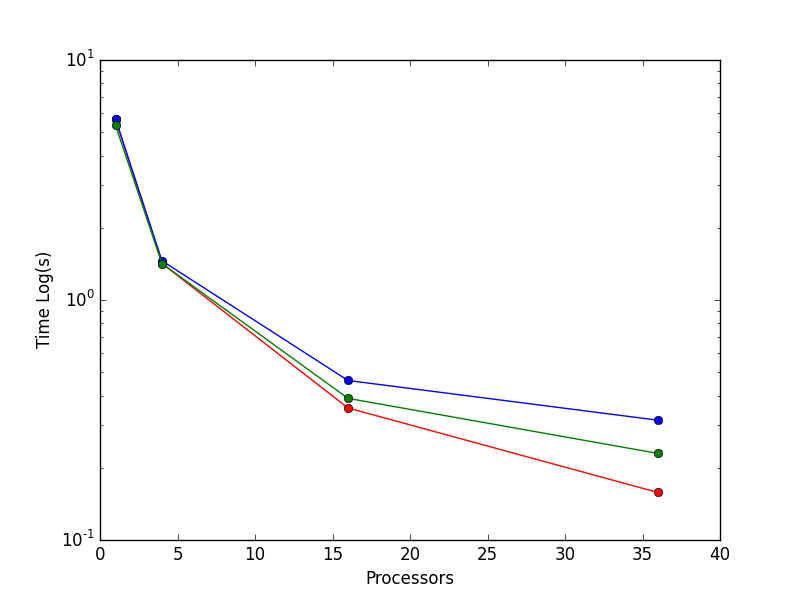
\includegraphics[width=.99\textwidth]{../2 Analysis/1000.png}
        \caption{$n = 1000$}
        \label{fig:1000}
      \end{subfigure}%
      \begin{subfigure}{.5\textwidth}
        \centering
        % 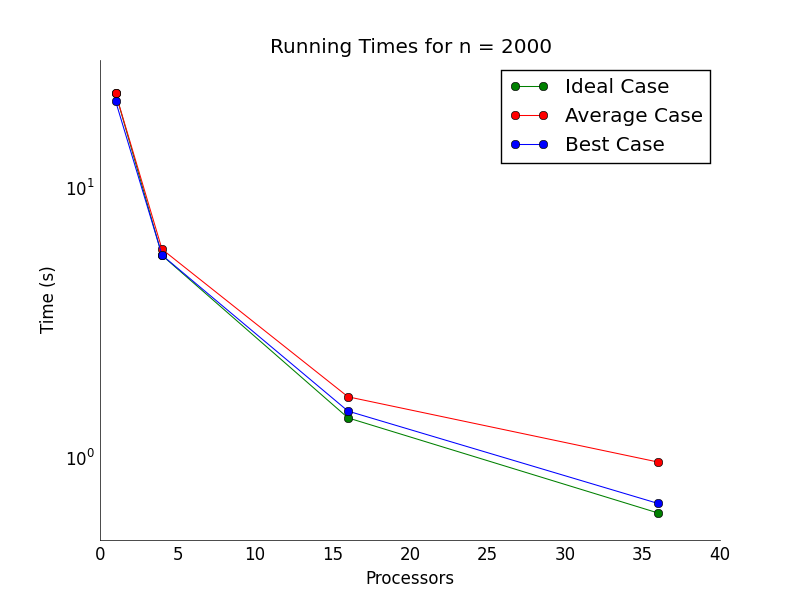
\includegraphics[width=.99\textwidth]{../2 Analysis/2000.png}
        \caption{$n = 2000$}
        \label{fig:2000}
      \end{subfigure}
      \caption{Logarithmic plot of times for different number of processors}
    \end{figure}

    Now, to analyze both SpeedUp and Efficiency, we can see the plots shown in Figures \ref{fig:SpeedUp} and \ref{fig:Efficiency}, in which we can find the ideal case, for $n = 1000$ and for $n = 2000$. In this plots an average of the minimum cases has been used to avoid deviating the data with longer timings.

    Analyzing the Figures we can see that we have achieved almost linear SpeedUp as the Equation \eqref{eq:SpeedUp} predicted. As $n$ goes from $1000$ to $2000$ the SpeedUp improves verifying our predictions. For the Efficiency, Equation \eqref{eq:Efficiency} predicted constant efficiency as $n$ grew larger. Figure \ref{fig:Efficiency} confirms this, with $n = 2000$ having a behavior much closer to ideal efficiency than $n = 1000$.

    Finally, it is important to notice that MPI communication does not behave as the theoretical models and therefore the results will not match perfectly to the model. Nevertheless, we have achieved successful results in the time needed to solve the problem.


    \begin{figure}[htp!]
      \centering
      \begin{subfigure}{.5\textwidth}
        \centering
        % 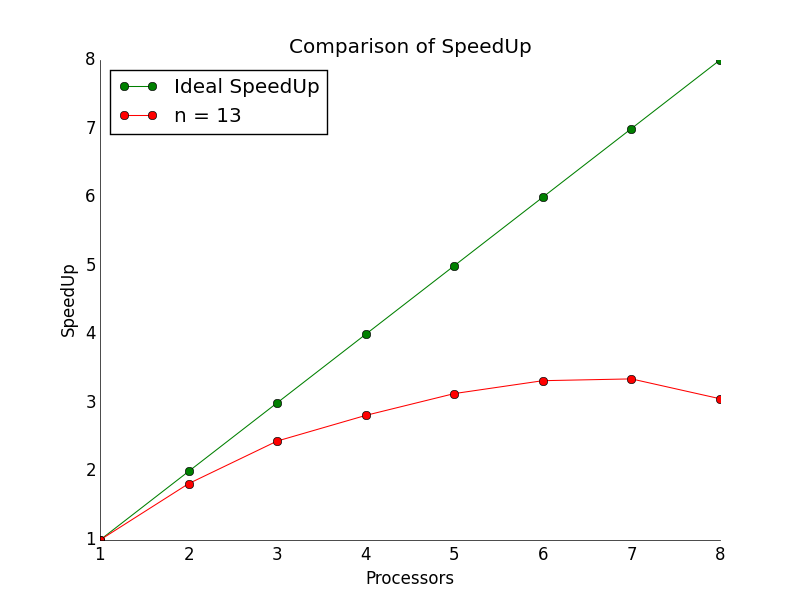
\includegraphics[width=.99\textwidth]{../2 Analysis/SpeedUp.png}
        \caption{Speed-Up}
        \label{fig:SpeedUp}
      \end{subfigure}%
      \begin{subfigure}{.5\textwidth}
        \centering
        % 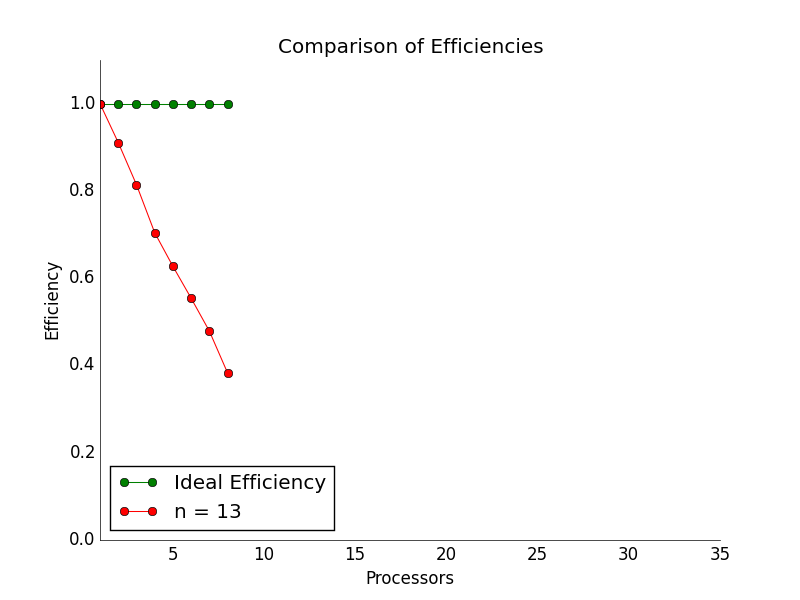
\includegraphics[width=.99\textwidth]{../2 Analysis/Efficiency.png}
        \caption{Efficiency}
        \label{fig:Efficiency}
      \end{subfigure}
      \caption{Speed-Up and Efficiency plots for the ideal case, $n=1000$ and $n = 2000$}
    \end{figure}



\end{document}
